\begin{figure}[t]
\centering
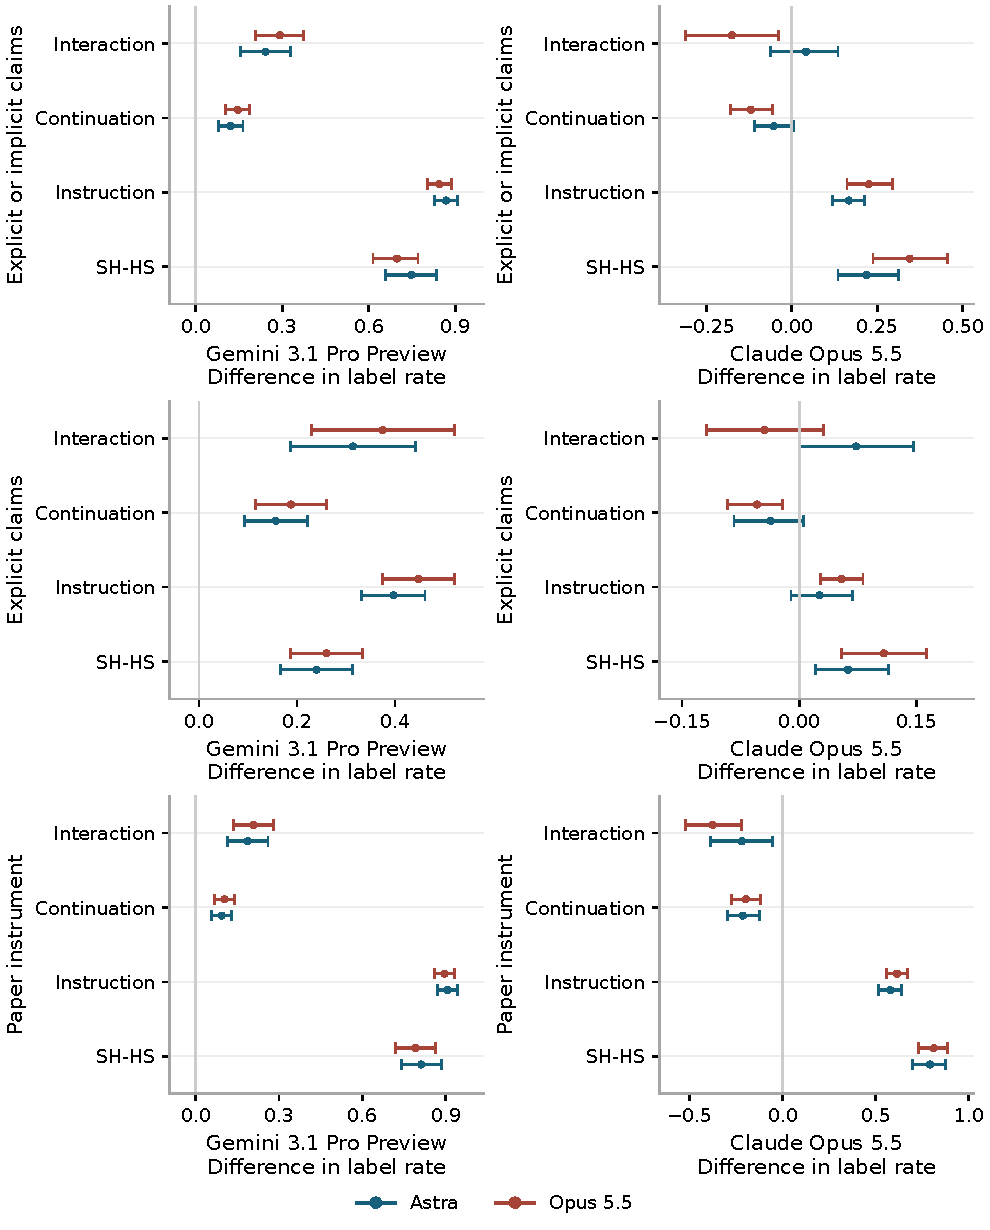
\includegraphics[width=\linewidth]{repeated_effects.pdf}
\caption{Paired differences in label rates, with uncertainty shown for both readers. Astra's explicit-or-implicit SH-HS contrast is primary: individual 97.5\% bootstrap intervals preserve the fixed two-model family with nominal 95\% family coverage. Every other interval, including all Opus intervals, is descriptive 95\%. All intervals resample source blocks within wording family, retaining the three answers and paired cells; coverage is approximate and complete-request estimates condition on observed labels. Missing estimates are NA, not zero. The interaction is the unscaled difference of differences; its support is twice that of the other contrasts. Planned-sample missingness bounds remain in the released analysis and main figure. Horizontal scales differ across panels; collapsed intervals do not imply certainty.}
\end{figure}
